\begin{singlespace}
\chapter[Supplementary Material for ``Causal single-cell RNA-seq simulation, in silico perturbation, and GRN inference benchmarking using GRouNdGAN-Toolkit'']{Supplementary Material for ``Causal single-cell RNA-seq simulation, in silico perturbation, and GRN inference benchmarking using GRouNdGAN-Toolkit''}
\markboth{Appendix B. Supplementary Material for GRouNdGAN-Toolkit}{Appendix B. Supplementary Material for GRouNdGAN-Toolkit}%
\end{singlespace}

\setcounter{table}{0}
\renewcommand{\thetable}{S\arabic{table}}
\renewcommand{\thefigure}{S\arabic{figure}}
\figuresection{Supplementary Material for ``Causal single-cell RNA-seq simulation, in silico perturbation, and GRN inference benchmarking using GRouNdGAN-Toolkit''}

\section*{Supplementary Methods}\label{sec:intrepppid_supp_methods}
\subsection*{Preparing strict PPI datasets}
A \textsc{ppi} dataset $\mathcal{D}$ is a set of interacting protein-pairs reflecting binary interactions $D_i \in \mathcal{D}$. $\mathcal{D}$ is partitioned into three mutually disjoint subsets: a training subset ($\mathcal{D}_\textrm{Tr}$), a testing subset ($\mathcal{D}_\textrm{Te}$), and a validation subset ($\mathcal{D}_\textrm{V}$). Let $P_\textrm{Tr}$, $P_\textrm{Te}$, and $P_\textrm{V}$ be the set of proteins present in $\mathcal{D}_\textrm{Tr}$, $\mathcal{D}_\textrm{Te}$, and
$\mathcal{D}_\textrm{V}$, respectively, and let $\mathcal{P}$ be the collection of protein sets ${P_\textrm{Tr}, P_\textrm{Te},  P_\textrm{V}}$.

We define a strict \textsc{ppi} dataset as a dataset $\mathcal{D}$ (with its collection of protein sets $\mathcal{P}$) that fulfills the following two criteria.

\textit{Criterion 1 --- Distinct Protein Identity}\\
The resulting protein sets $P_\textrm{Tr}, P_\textrm{Te},  P_\textrm{V}$ of the dataset must be mutually disjoint:

$$
\forall Q, R \in \mathcal{P} \; Q \cap R = \emptyset \; \textrm{if} \; Q \neq R.
$$

\textit{Criterion 2 --- Distinct Sequence Identity}\\
The amino acid sequence of any pair of proteins belonging to different protein subsets must have a sequence identity no greater than 90\%:

$$
\forall Q, R \in \mathcal{P}, \; \forall q \in Q \; \forall r \in R \; f(q,r) \leq 90\% \; \textrm{if} \; Q \neq R
$$

where $f(\cdot,\cdot)$ is some protein sequence identity function.

For the datasets used in the experiments carried out herein, the UniRef90 identifiers provided by UniProt were used to determine sequence identity, and as such we adopt the same definition of sequence identity [1,2].

\textit{High-confidence examples of \textsc{ppi}s}\\
To minimize our exposure to falsely labelled \textsc{ppi}s, we required a database that provided information regarding the confidence of the interactions. We selected the \textsc{string} database as the source of \textsc{ppi}s for our datasets as it is large, contains information for many species, and integrates confidence scores from a number of modalities [3]. We exclude all \textsc{ppi}s which do not have a combined confidence score greater or equal to 90\%, and only include \textsc{ppi}s which are
classified as ``physical interactions''. \textsc{ppi} information for seven species were included in our analyses.

\begin{table}[h]
	 {\begin{tabular}{@{}llll@{}}\toprule 
			Scientific Name & Common Name & \textsc{ncbi} Taxon \textsc{id} & Patristic Distance\\
                            &                &                     & from \textit{H.~sapiens}\\\midrule
			\textit{Homo sapiens} & Human & 9606 & 0.000 \\
            \textit{Mus musculus} & House mouse & 10090 & 0.0455 \\
            \textit{Danio rerio} & Zebrafish & 7955 & 0.156 \\
            \textit{Drosophila melanogaster} & Fruit fly & 7227 & 0.358 \\
            \textit{Caenorhabditis elegans} & Nematode & 6239 & 0.455 \\
            \textit{Arabidopsis thaliana} & Thale cress & 3702 & 0.693 \\
            \textit{Saccharomyces cerevisiae} & Baker's yeast & 4932 & 0.734 \\
			\midrule
	\end{tabular}}{}
\end{table}

Patristic distance is a measure of the divergence of two lineages. Patristic distances were computed using DendroPy and data from i\textsc{tol} [4,5].

\textit{Negative examples of \textsc{ppi}s}\\
As \textsc{intrepppid} is a supervised method, it requires examples of pairs of proteins which do not interact (negative examples), in addition to pairs which do (positive examples). Obtaining negative examples of \textsc{ppi}s is a fraught process as there exists no one agreed upon ``gold standard'' of proteins which do not interact with one another. While many approaches for obtaining negative \textsc{ppi} examples have been devised over the years, evidence has shown that many of these methods introduce a great amount of bias [6]. For this reason, we opted to sample pairs of proteins in a uniformly random manner to represent our negative examples. For the training set, negatives were randomly drawn without replacement from the set $N_\textrm{Tr}$, defined as:

$$
N_\textrm{Tr} = \left\{\{p,q\} | p \in P_\textrm{Tr}, q \in P_\textrm{Tr}, \{p,q\} \notin \mathcal{D} \right\}
$$

Negative examples for the testing and validation sets were drawn from $N_\textrm{Te}$ and $N_\textrm{V}$, which were similarly defined as the set of protein-pairs of $P_\textrm{Te}$ and $P_\textrm{V}$, respectively, which were not in $\mathcal{D}$ (\textit{i.e.}, were not considered interacting in the dataset).

Random sampling of protein-pairs requires the fewest assumptions about the distribution of negative pairs, thereby reducing bias, albeit at the risk of false-negatives. Through the exclusion of known interactions from $N_\textrm{Tr}$, however, we’ve reduced the likelihood of drawing false-negatives.

\textit{Considerations for cross-species datasets}\\
For experiments herein, it was necessary to prepare datasets suitable for testing the cross-species task. Namely, we needed to construct training sets whose \textit{ppi}s were composed of proteins of one species, and many corresponding testing sets each belonging to a different species. All combinations of the training set and the many testing sets must satisfy both Criteria 1 and 2. The first criterion is typically met \textit{de facto}, as protein identifiers between species normally do not overlap. In order for the second criterion to be met, positive and negative interactions of proteins that do not satisfy Criterion 2 were excluded from the datasets.
\newpage
\section*{Supplementary Tables and Figures}
\subsection*{Tables}

\subsubsection*{Table S1}
\label{sec:intrepppid_supp_s1}

Table S1 is provided as a separate .xlsx spreadsheet file.
\addtocounter{table}{1}

Its caption is as follows:

\begin{displayquote}
\begin{singlespace}
Statistics of each dataset used in this study. Datasets are listed by source organism and random seed used to generate the random splits.
\end{singlespace}
\end{displayquote}

\begin{tcolorbox}
    This file is available for download from \textsc{oup} Briefings in Bioinformatics:\\ \href{https://doi.org/10.1093/bib/bbae405}{https://doi.org/10.1093/bib/bbae405}.
\end{tcolorbox}

\newpage

\begin{table}[!h]
\centering
	\caption[Hyperparameters used to train \textsc{intrepppid} in all experiments.]{\textsf{\textbf{Hyperparameters used to train INTREPPPID in all experiments.}}} \label{tab:intrepppid_supp_hyperparameters} {\begin{tabular}{@{}ll@{}}\toprule 
			Hyperparameter & Value  \\\midrule
			Batch Size & 80 \\
            Embedding Size & 64 \\
            Number of \textsc{rnn} Layers & 2 \\
            \textsc{rnn} Drop-connect Rate & 0.3 \\
            Embedding Drop-out Rate & 0.3\\
			\midrule
	\end{tabular}}{}

\end{table}

\newpage

\subsubsection*{Table S3}
\label{sec:intrepppid_supp_s3}

Table S3 is provided as a separate .xlsx spreadsheet file.
\addtocounter{table}{1}

Its caption is as follows:

\begin{displayquote}
\begin{singlespace}
Confusion matrix statistics of various methods trained and tested on \textit{H.~sapiens} data.
\end{singlespace}
\end{displayquote}

\begin{tcolorbox}
    This file is available for download from \textsc{oup} Briefings in Bioinformatics:\\ \href{https://doi.org/10.1093/bib/bbae405}{https://doi.org/10.1093/bib/bbae405}.
\end{tcolorbox}

\newpage
\begin{table}[!h]
\centering
	\caption[Performance of \textsc{intrepppid} tested on increasing negative-to-positive ratios.]{\textsf{\textbf{Performance of INTREPPPID trained on \textit{H.~sapiens} datasets with a 1:1 negative-to-positive interaction ratios, and tested on increasing negative-to-positive ratios.}}} \label{tab:intrepppid_supp_neg_ratio} {\begin{tabular}{@{}llllll@{}}\toprule 
			Negative:Positive & 1:1 & 2:1 & 10:1 & 50:1 & 100:1  \\\midrule
			\textsc{auroc} Mean & 0.752 & 0.723 & 0.733 & 0.728 & 0. 733 \\
            \textsc{auroc} Std & 0.017 & 0.004 & 0.006 & 0.011 & 0.004\\
			\midrule
	\end{tabular}}{}

\end{table}

\newpage

\subsubsection*{Table S5}
\label{sec:intrepppid_supp_s5}

Table S5 is provided as a separate .xlsx spreadsheet file.
\addtocounter{table}{1}

Its caption is as follows:

\begin{displayquote}
\begin{singlespace}
Metrics of various \textsc{ppi} inference methods trained on \textit{H.~sapiens} data, and tested on various species. Each model was tested on a total of twenty-four dataset: four different random testing splits for each six different organism. The metrics reported here are averaged over all four datasets, with the standard deviation between the four datasets also reported. The first worksheet (\textsc{auroc}) reports the area-under-the-receiver-operator-curve (\textsc{auroc}). The second worksheet (\textsc{ap}) reports the average-precision. The third worksheet (F150) reports the $F_1$ measure with a 50\% threshold.
The fourth worksheet (MCC50) reports the Matthew's correlation coefficient (\textsc{MCC}) with a 50\% threshold. The fifth and final worksheet (Brier) reports the Brier score. Higher values indicate better performance for all metrics but the Brier score, where the inverse is true.
\end{singlespace}
\end{displayquote}

\begin{tcolorbox}
    This file is available for download from \textsc{oup} Briefings in Bioinformatics:\\ \href{https://doi.org/10.1093/bib/bbae405}{https://doi.org/10.1093/bib/bbae405}.
\end{tcolorbox}

\newpage

\begin{table}[!h]
\centering
	\caption[Performance of \textsc{intrepppid} with scrambled and not scrambled orthologue information.]{\textsf{\textbf{Performance of INTREPPPID trained on \textit{H.~sapiens} datasets with scrambled and not
scrambled orthologue information.}} Bold-face indicates the best value for each metric.} \label{tab:intrepppid_supp_scramble} {\begin{tabular}{@{}lllll@{}}\toprule 
			Scramble Status & Test \textsc{auroc} & Test \textsc{ap} & Test \textsc{mcc}@50\% & Test Brier Score  \\\midrule
			Not Scrambled & \textbf{0.761} & \textbf{0.737} & \textbf{0.378} & \textbf{0.198} \\
            Scrambled & 0.524 & 0.527 & 0.017 & 0.314 \\
			\midrule
	\end{tabular}}{}

\end{table}

\newpage

\begin{table}[!h]
\centering
	\caption[Change in \textsc{intrepppid} performance when omitting orthology data.]{\textsf{\textbf{Performance of INTREPPPID when trained on \textit{H.~sapiens} dataset which omits orthology data for the seven species tested below, relative to the performance of INTREPPPIED trained on dataset which includes all orthology data available.}}} \label{tab:intrepppid_supp_no_ortho} {\begin{tabular}{@{}lllll@{}}\toprule 
			Testing Dataset & Test \textsc{auroc} & Test \textsc{ap} & Test \textsc{mcc}@50\% & Test Brier Score  \\\midrule
			\textit{H.~sapiens} & -0.49\% & -1.36\% & -9.00\% & 2.00\% \\
            \textit{M. musculus} & -13.21\% & -14.79\% & 34.39\%  & 21.06\% \\
            \textit{D. rerio} & -13.69\% & -16.16\% & -38.85\%  & 8.66\% \\
            \textit{D. melanogaster} & -11.29\% & -11.67\% & -26.48\%  & 5.81\% \\
            \textit{C. elegans} & -12.51\% & -17.58\% & -13.45\%  & -0.73\% \\
            \textit{S. cerevisiae} & -9.21\% & -15.12\% & -13.31\%  & -3.17\% \\
            \textit{A. thaliana} & -9.29\% & -11.55\% & -30.75\%  & 5.39\% \\
			\midrule
	\end{tabular}}{}
\end{table}

\newpage

\subsubsection*{Table S8}
\label{sec:intrepppid_supp_s8}

Table S8 is provided as a separate .xlsx spreadsheet file.
\addtocounter{table}{1}

Its caption is as follows:

\begin{displayquote}
\begin{singlespace}
Results of the statistical over-expression analysis conducted on top \textsc{intrepppid}-unique positive hits for seven species. The statistical over-expression of \textsc{go} Molecular Function annotations among proteins that make up the top \textsc{intrepppid}-unique positive hits was measured relative to the proteins which make up the testing dataset for the specific species tested. A Fisher's Exact test was performed by the online \textsc{panther} Classification System. The fold enrichment, raw $p$ values, and corrected $p$ values using Benjamini-Hochberg false-discover rate (\textsc{fdr}) correction are reported for \textsc{go} Molecular Function annotations found to be over-expressed. Only results with a corrected $p$ value of less than 0.05 are included in this table. Each worksheet in the spreadsheet is labelled with a species name, and reports the over-expression analysis for the testing dataset that belongs to that species.
\end{singlespace}
\end{displayquote}

\begin{tcolorbox}
    This file is available for download from \textsc{oup} Briefings in Bioinformatics:\\ \href{https://doi.org/10.1093/bib/bbae405}{https://doi.org/10.1093/bib/bbae405}.
\end{tcolorbox}

\newpage

\begin{table}[!h]
\centering
	\caption[Analysis of online availability of \textsc{ppi}-related tools.]{\textsf{\textbf{Analysis of 22 randomly sampled articles advertising online PPI-related tools and the online availability of said tools as of January 2024.}} Articles were found using the SemanticScholar.org academic search engine with the search terms ``protein-protein interaction website''.} \label{tab:intrepppid_supp_links} {\begin{tabular}{@{}lllll@{}}\toprule 
			\textsc{doi} & Corpus\textsc{id} & Year Published & \textsc{uri} & Status  \\\midrule
			\texttt{10.1093/nar/gks434} & 9914396 & 2012 & \href{http://dropnet.isima.fr/}{Link} & \textcolor{red}{Dead} \\
            \texttt{10.1007/978-1-0716-0892-0\_12} & 226218388 & 2020 & \href{http://wodaklab.org/iRefWeb}{Link} & \textcolor{ForestGreen}{Alive} \\
            \texttt{10.1007/978-1-4939-9873-9\_12} & 203659921 & 2020 & \href{https://oncoppi.emory.edu/}{Link} & \textcolor{ForestGreen}{Alive} \\
            \texttt{10.1515/jib-2006-27} & 16195629 & 2006 & \href{http://biomis.fh-hagenberg.at/isp/primos}{Link} & \textcolor{red}{Dead} \\
            \texttt{10.1089/adt.2013.506} & 12969509 & 2013 & \href{http://primos.fh-hagenberg.at/}{Link} & \textcolor{red}{Dead} \\
            \texttt{10.1093/nar/gkx333} & 31083221 & 2017 & \href{https://proteins.plus/}{Link} & \textcolor{ForestGreen}{Alive} \\
            \texttt{10.1371/journal.pone.0056228} & 2014834 & 2013 & \href{http://www.canevolve.org/}{Link} & \textcolor{red}{Inaccessible\textsuperscript{1}} \\
            \texttt{10.1093/nar/gkp335} & 3041302 & 2009 & \href{https://meme.nbcr.net/}{Link} & \textcolor{red}{Inaccessible\textsuperscript{2}} \\
            \texttt{10.1093/NAR/GKG056} & 15003973 & 2003 & \href{http://www.bind.ca/}{Link} & \textcolor{red}{Dead} \\
            \texttt{10.1109/CBMS.2008.113} & 19040991 & 2009 & \href{http://212.189.149.159:8080/mcl_service}{Link} & \textcolor{red}{Dead} \\
            \texttt{10.1093/nar/gkx385} & 3268569 & 2017 & \href{http://dynomics.pitt.edu/}{Link} & \textcolor{ForestGreen}{Alive} \\
            \texttt{10.1093/nar/gkac1000} & 253479599 & 2022 & \href{https://string-db.org/}{Link} & \textcolor{ForestGreen}{Alive} \\
            \texttt{10.7726/AJBCB.2014.1003} & 12004796 & 2014 & \href{http://bicompute.appspot.com/}{Link} & \textcolor{ForestGreen}{Alive} \\
            \texttt{10.1093/bioinformatics/btn584} & 206340817 & 2009 & \href{http://www.bioinformatics.sussex.ac.uk/protorp}{Link} & \textcolor{red}{Dead} \\
            \texttt{10.1186/1471-2105-11-S10-P1} & 40906621 & 2010 & \href{http://www.compbio.dundee.ac.uk/pips}{Link} & \textcolor{ForestGreen}{Alive} \\
            \texttt{10.1093/bioinformatics/btx312} & 4420839 & 2017 & \href{https://www.iitm.ac.in/bioinfo/PROXiMATE/}{Link} & \textcolor{ForestGreen}{Alive} \\
            \texttt{10.1155/2013/737591} & 5548876 & 2013 & \href{http://nrf2.elte.hu/}{Link} & \textcolor{red}{Dead} \\
            \texttt{10.1038/nmeth.1931} & 52853893 & 2012 & \href{http://www.imexconsortium.org/}{Link} & \textcolor{ForestGreen}{Alive} \\
            \texttt{10.3389/fgene.2021.722198} & 229549097 & 2020 & \href{https://rbc-dsai-iitm.github.io/NetGenes/}{Link} & \textcolor{ForestGreen}{Alive} \\
            \texttt{10.1093/nar/gkv1072} & 8843610 & 2015 & \href{https://www.bindingdb.org/rwd/bind/index.jsp}{Link} & \textcolor{ForestGreen}{Alive} \\
            \texttt{10.1093/nar/gkt1210} & 560515 & 2013 & \href{https://ipfam.org/}{Link} & \textcolor{red}{Dead} \\
			\midrule
	\end{tabular}}{}
\end{table}

\textsuperscript{1}Presents a login page with no context or registration option.\\
\textsuperscript{2}URI resolves but the described online web server is not present.

\newpage
\subsection*{Figures}

\begin{figure}[h]
	\centerline{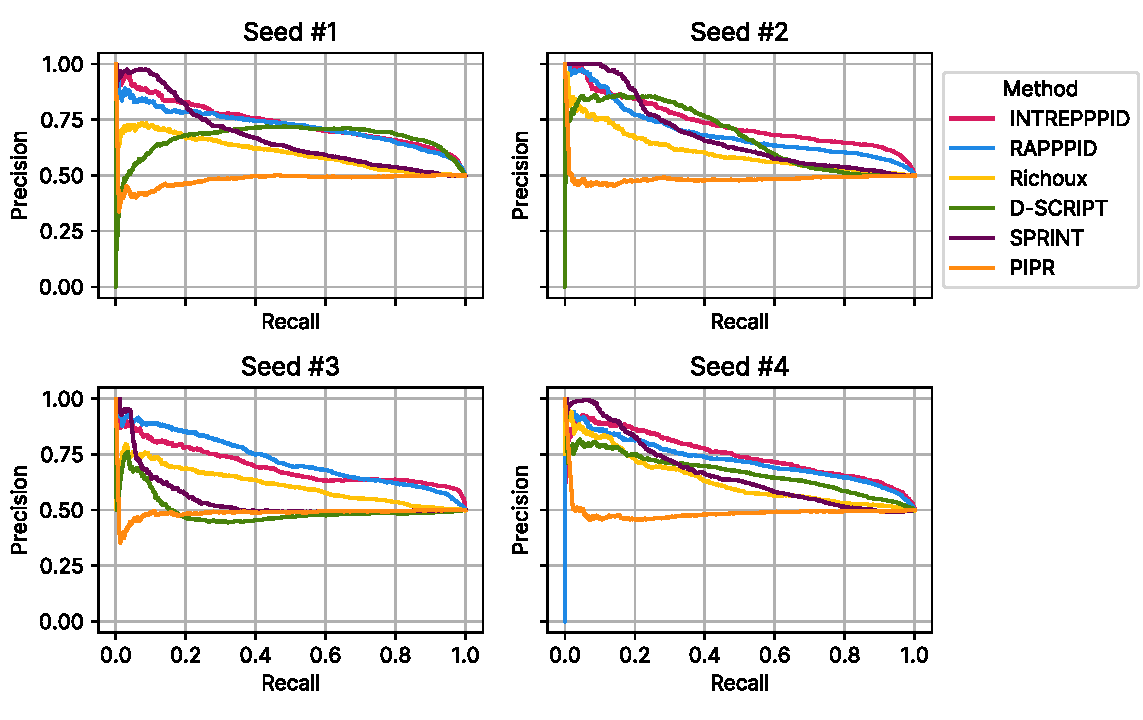
\includegraphics[scale=0.8]{figures/intrepppid/pr_curve3.pdf}}
	\caption[Precision-Recall curves of various \textsc{ppi} inference methods]{\textsf{\textbf{Precision-Recall curves of various PPI inference methods tested and trained on \textit{H.~sapiens} data.}} Each panel reports the Precision-Recall curve for one of four different datasets.}\label{fig:intreppid_supp_pr}
\end{figure}

\begin{figure}[h]
	\centerline{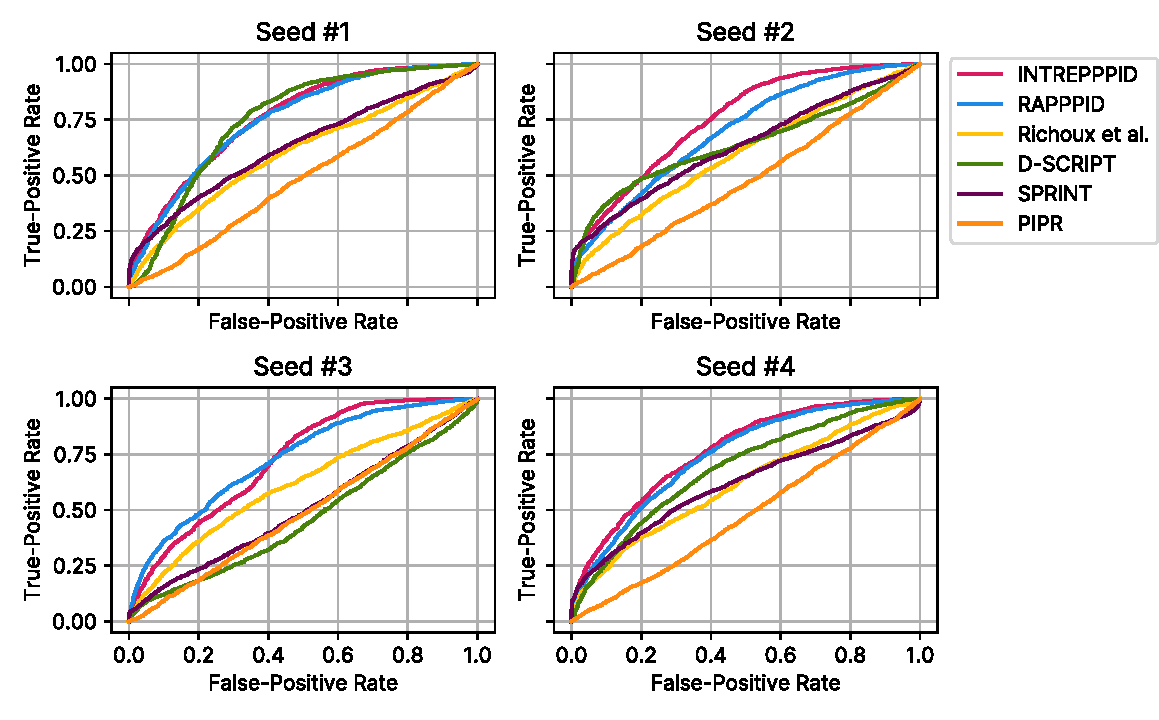
\includegraphics[scale=0.8]{figures/intrepppid/roc3.pdf}}
	\caption[Receiver-Operator curves of various \textsc{ppi} inference methods]{\textsf{\textbf{Receiver-Operator curves of various PPI inference methods tested and trained on \textit{H.~sapiens} data.}} Each panel reports the Receiver-Operator curve for one of four different datasets.}\label{fig:intreppid_supp_roc}
\end{figure}

\begin{figure}[h]
	\centerline{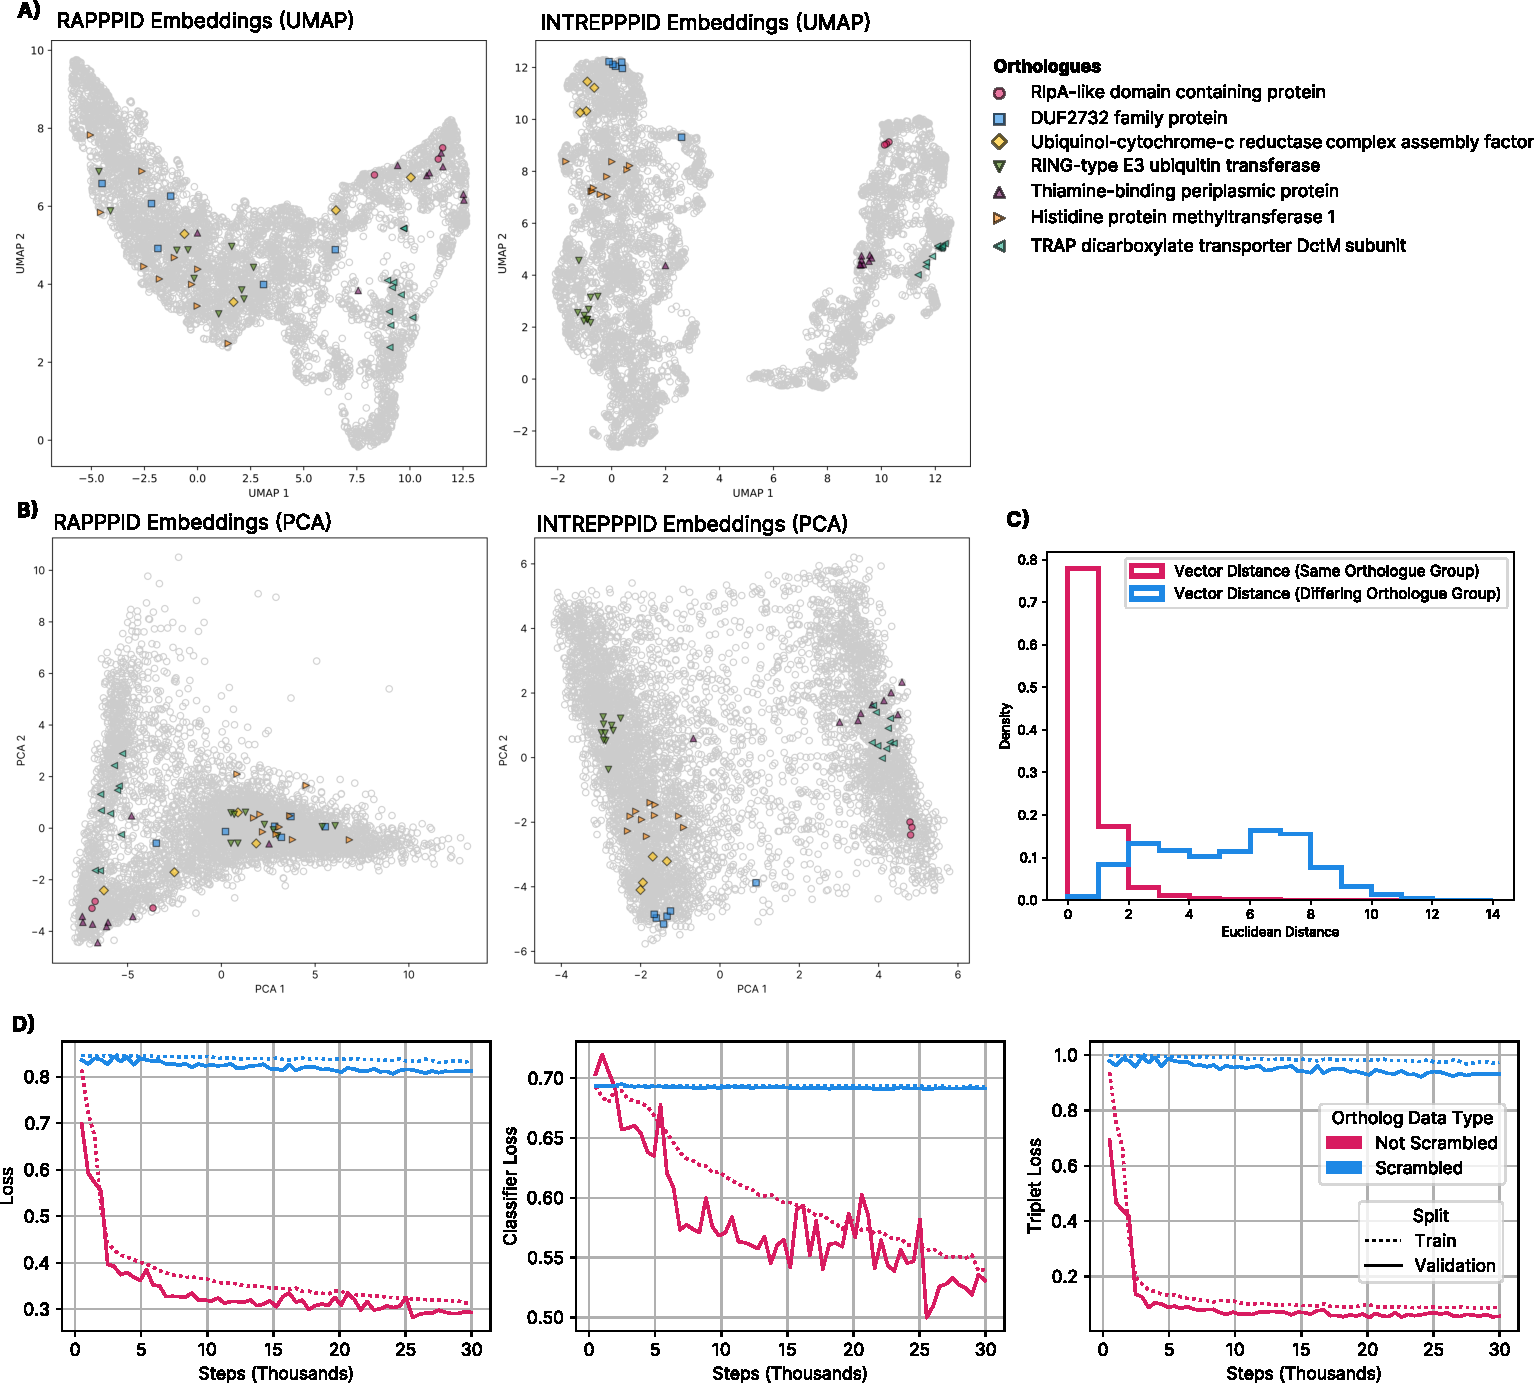
\includegraphics[scale=0.6]{figures/intrepppid/scramble_oma4.pdf}}
	\caption[The effect of orthologous locality task.]{\textsf{\textbf{The effect of orthologous locality task.}} \textbf{(A-B)} A random sample of protein sequences
from various species were embedded using \textsc{rapppid} (left) and \textsc{intrepppid} (right) and projected onto a 2D space using the \textbf{(A)} \textsc{umap} and \textbf{(B)} \textsc{pca} algorithm. Distinct markers indicate proteins which belong to the same orthologous group according to the \textsc{oma} database. The orthologous groups shown were chosen at random. \textbf{(C)} Histogram of the Euclidean distance between \textsc{intrepppid} latent vector representations of protein sequences of the same orthologous group (magenta) and of differing orthologous groups (blue). \textbf{(D)} Training (dotted line) and validation loss (solid line) of \textsc{intrepppid} trained on \textit{H.~sapiens} datasets whose orthologue data is ``scrambled'' (blue) and ``not scrambled'' (magenta). The overall loss (left), the loss of the classification network (middle), and the loss of the triplet network (right) are plotted above, demonstrating that the ``scrambled'' dataset fails to optimize any aspect of the loss in any appreciable way.}\label{fig:intreppid_supp_scramble} \end{figure}
\clearpage
\section*{References}
\begin{enumerate}
    \item  Suzek BE, Wang Y, Huang H, \textit{et al.} UniRef clusters: a comprehensive and scalable alternative for improving sequence similarity searches. \textit{Bioinformatics} 2015; 31:926–932
    
    \item The UniProt Consortium, Bateman A, Martin M-J, \textit{et al.} UniProt: the Universal Protein Knowledgebase in 2023. \textit{Nucleic Acids Research} 2023; 51:D523–D531

    \item Szklarczyk D, Kirsch R, Koutrouli M, \textit{et al.} The \textit{string} database in 2023: protein–protein association networks and functional enrichment analyses for any sequenced genome of interest. \textit{Nucleic Acids Research} 2023; 51:D638–D646

    \item Sukumaran J, Holder MT. DendroPy: a Python library for phylogenetic computing. \textit{Bioinformatics} 2010; 26:1569–1571

    \item Letunic I, Bork P. Interactive Tree Of Life (i\textsc{tol}) v5: an online tool for phylogenetic tree display and annotation. \textit{Nucleic Acids Research} 2021; 49:W293–W296

    \item Ben-Hur A, Noble WS. Choosing negative examples for the prediction of protein-protein interactions. \textit{BMC Bioinformatics} 2006; 7:S2–S2
\end{enumerate}